\documentclass[8pt,a4paper,twoside,onecolumn,leqno,fleqn]{article}

\newcommand{\HRule}{\rule{\linewidth}{0.5mm}}
\usepackage[utf8]{inputenc}
\usepackage[french,english]{babel}
\usepackage[T1]{fontenc}
\usepackage{amsmath,amsthm,amsfonts,amssymb,mathtools}
\usepackage{graphicx}
\usepackage{adjustbox}
\usepackage{subcaption}
\usepackage{float}
\usepackage{color}
\usepackage[table,xcdraw]{xcolor}
\definecolor{silver}{rgb}{0.75, 0.75, 0.75}
\usepackage{tikz}
\usetikzlibrary{arrows.meta, positioning, fit, calc, shapes, patterns}
% \usetikzlibrary{shapes.geometric}
\usepackage{hyperref}
%\usepackage[addtotoc]{abstract}
\usepackage[left=2cm,right=2cm,top=2cm,bottom=2cm]{geometry}
\usepackage{fancyhdr}
\pagestyle{fancy}
\usepackage{url}
\usepackage{varioref}
\usepackage{cleveref}
\usepackage{hyperref}
\usepackage{nameref}
\usepackage{titleref}
\usepackage{lettrine}
\usepackage{tabto}
\usepackage{longtable}
\usepackage{lipsum}
\usepackage{siunitx}
\usepackage{multirow}
\usepackage{booktabs}
\usepackage{tabularx}
\usepackage{array}
\usepackage{algorithm}
\usepackage{algpseudocode}
\usepackage{caption}
\captionsetup[table]{labelsep=space, justification=centering}
\usepackage{diagbox}

% GLOSSARY
% \usepackage[acronym,toc]{glossaries}
\usepackage[acronym,nomain,toc]{glossaries}
\makeglossaries
\loadglsentries{Pages/Glossary/glossary.tex}

%\usepackage{pgfplots}
\sisetup{
	round-mode          = places, % Rounds numbers
	round-precision     = 2, % to 2 places
}
\usepackage[
type={CC},
modifier={by-nc-sa},
version={4.0},
]{doclicense}
%header
\renewcommand{\headrulewidth}{1pt}
\fancyhead[C]{} 
\fancyhead[L]{\leftmark}
\fancyhead[R]{\rightmark}
%footer
\renewcommand{\footrulewidth}{1pt}
\fancyfoot[C]{\textbf{page \thepage}} 
\fancyfoot[L]{\doclicenseNameRef
	— \copyright Baptiste Grosjean}
\fancyfoot[R]{Ann\'eee acad\'emique 2023-2024}
%bibilography
\usepackage[backend=biber,natbib=true,sortcites=true,style=numeric,sorting=none]{biblatex}
\usepackage[babel=true,autostyle=true]{csquotes}
%\renewcommand{\thesection}{\Roman{section}}
\author{Baptiste Grosjean}
\title{}
\date{\today}

\addbibresource{./Sources/Sources.bib}

\begin{document}
\hypersetup{hidelinks}
\setlength{\parskip}{6pt}
\setlength{\headheight}{14.61858pt}
\addtolength{\topmargin}{-2.49998pt}

\begin{titlepage}

	\begin{center}
	% Partie supérieure de la page
	
\includegraphics[width=0.3\textwidth]{./Images/Logos/fs.pdf}\hfill
	
\includegraphics[width=0.5\textwidth]{./Images/Logos/umons_charleroi.png}\\[1cm]
	
	{\LARGE Université de Mons}\\[0.5cm]
	{\Large Faculté des Sciences}\\[1cm]
	
	{\Large US-MC-INFO60-014-C — Lecture et rédaction scientifique}\\[1cm]
	
	% Titre
	\HRule \\[0.4cm]
	{ \Huge \bfseries TOR:}\\[0.2cm]
	{ \LARGE \bfseries Le Routage Onion de Seconde Génération}\\[0.4cm]
	\HRule \\[1.5cm]
	
	% Auteur et directeur
	\begin{minipage}{0.4\textwidth}
	\begin{flushleft} \large
	\emph{Auteur:}\\
	Baptiste \textsc{Grosjean}
	\end{flushleft}
	\end{minipage}
	~
	\begin{minipage}{0.4\textwidth}
	\begin{flushright} \large
	\emph{Directeur:}\\
	Alain \textsc{Buys}
	\end{flushright}
	\end{minipage}\\[2cm]
	
	\begin{minipage}{0.4\textwidth}
	\begin{flushleft} \large
	\emph{Numéro d'étudiant:}\\
	232732
	\end{flushleft}
	\end{minipage}\\[2cm]
	
	% Résumé
	\renewcommand{\abstractname}{Résumé}
	\begin{abstract}
	\acrfull{tor} est un système de communication sécurisé et fiable. Ce travail de rédaction scientifique vise à fournir une compréhension détaillée du protocole \acrshort{tor}, de son fonctionnement et de son importance dans les réseaux modernes. Nous utiliserons \LaTeX\ pour produire une documentation claire et précise du protocole ainsi que de son implémentation pratique.
	\end{abstract}
	
	\vfill
	
	% Bas de la page
	{\large Juin 2024}
	\end{center}
	\end{titlepage}


\newpage
\setcounter{page}{1}
\thispagestyle{empty}
\mbox{}

\newpage
\thispagestyle{empty}
\renewcommand{\contentsname}{Sommaire}
\tableofcontents

\newpage
\section{Introduction}\label{sec:introduction}
\subsection{Vue d'ensemble}

Un système d'exploitation est constitué d'un noyau auquel vient s'ajouter le code d'une distribution.
Le développeur d'un système d'exploitation doit abstraire le fonctionnement des périphériques afin d'offre un interface de programmation au programmeur.
La gestion des ressources et les communications avec les différents périphériques est gérée par le système d'exploitation.

\subsection{Vue d'ensemble}
Le système d'exploitation (SE) est le logiciel de base qui gère les ressources matérielles et logicielles d'un ordinateur, offrant des services essentiels pour l'exécution des programmes. 
Un SE permet aux utilisateurs et aux applications d'interagir avec le matériel sans nécessiter de connaître les détails techniques sous-jacents.

\subsection{Abstractions de programmation}

Un système d’exploitation peut être perçu comme exposant une interface de programmation système aux programmes qui tournent sur une machine.

\begin{figure}[h!]
    \centering
    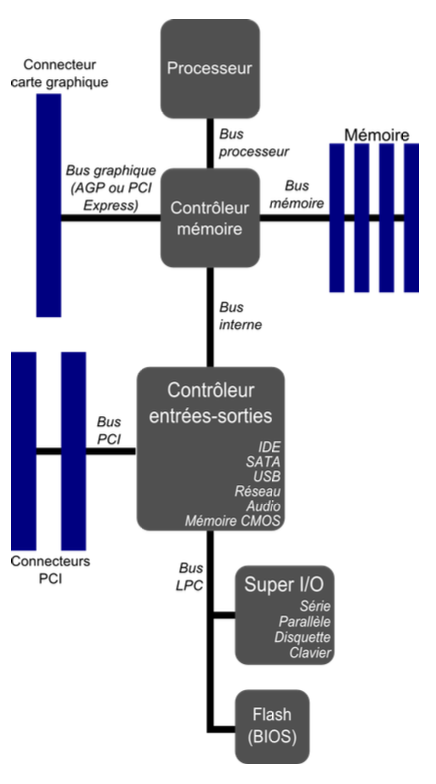
\includegraphics[width=0.2\textwidth]{Images/View/view.png}
    \caption{View}
    \label{fig:myimage}
  \end{figure}
  

\subsection{Processeur}


Le \textbf{processeur} exécute les instructions et réalise les traitements. 
Il est caractérisé par son jeu d'instructions (Instruction Set Architecture), qui définit les instructions exécutables et leur format d'encodage (opcode et opérandes). 
Les instructions sont classées en plusieurs types :
\begin{itemize}
    \item Arithmétique (e.g. \texttt{add}, \texttt{div})
    \item Logique (e.g. \texttt{and})
    \item Accès mémoire (e.g. \texttt{lw}, \texttt{sw})
    \item Instructions système
\end{itemize}

Les processeurs modernes utilisent une structure de pipeline, permettant à différentes instructions d'occuper simultanément différentes parties du pipeline. 
Deux types principaux d'architecture de jeu d'instructions existent :
\begin{itemize}
    \item RISC (Reduced Instruction Set Computer)
    \item CISC (Complex Instruction Set Computer)
\end{itemize}

Les responsabilités de gestion du processeur en collaboration avec le système d'exploitation incluent :
\begin{itemize}
    \item Surveillance de l'exécution des instructions
    \item Répartition du temps processeur entre différents programmes
\end{itemize}


\subsubsection{Exécution de programme}

La première responsabilité de gestion consiste à surveiller l'exécution des instructions d'un programme utilisant le processeur. 
Le système d'exploitation et les programmes se partagent le processeur, nécessitant la suspension de l'exécution en cours lors d'un évènement particulier. 
Le processeur peut réagir de différentes manières :

\begin{itemize}
    \item \textbf{Mauvais comportement} : déroutement vers une fonction du système d'exploitation pour traiter des erreurs telles qu'une division par zéro, un accès mémoire invalide ou une tentative d'exécuter une instruction privilégiée.
    \item \textbf{Anomalie non fatale} : correction des circonstances ayant provoqué l'anomalie et reprise de l'exécution.
    \item \textbf{Appel système} : branchement vers une fonction du système d'exploitation pour des demandes comme l'obtention de mémoire ou l'écriture dans un fichier.
    \item \textbf{Interruption externe} : traitement d'une interruption provenant d'un périphérique externe. 
    Par exemple, une interruption du clavier nécessite de communiquer avec le contrôleur du clavier pour identifier la touche concernée et le programme destinataire.
\end{itemize}


\subsubsection{Ordonnancement de programmes}

La seconde responsabilité du système d'exploitation est de répartir le temps processeur entre les programmes. 
L'ordonnancement sélectionne le prochain programme à exécuter lorsque le processeur est libre. 
Différentes stratégies sont utilisées selon le type de système et la charge de travail. 
Les métriques d'évaluation incluent la minimisation du temps d'exécution moyen et l'adéquation entre les besoins du programme et le temps processeur alloué.


\subsection{Mémoire}

La mémoire stocke les données de travail des programmes et est organisée en une hiérarchie :
\begin{itemize}
    \item \textbf{Caches} (e.g. L1, L2) : Intermédiaires entre les registres et la mémoire principale, stockant temporairement les données fréquemment accédées (principe de localité).
    \item \textbf{Mémoire principale} (e.g. RAM, GPU) : Stocke les données de travail (e.g. tableaux, variables, stack) lorsqu'il n'y a pas de registres disponibles.
    \item \textbf{Mémoire secondaire} (e.g. HDD, SSD) : Utilisée comme espace temporaire (swap) lorsque la mémoire principale est pleine.
\end{itemize}

L'allocation dynamique permet de gérer la mémoire de manière flexible. La mémoire virtuelle charge/décharge les données non actives pour pallier les limitations de la mémoire physique (e.g. adressage 32 bits, 0x00000000 à 0xffffffff).


\subsubsection{Protection de la mémoire}

Le système d'exploitation contrôle les accès mémoire pour garantir qu'un programme n'accède qu'à sa propre mémoire, évitant ainsi la lecture ou la modification de données sensibles (e.g. clefs de chiffrement). 
Le processeur vérifie les accès mémoire selon les descriptions des espaces mémoire accessibles à chaque programme, mises à jour par le système d'exploitation.

\begin{itemize}
    \item \textbf{Adresse valide} : Accessible au programme, l'accès est accordé (e.g. \texttt{lw}, \texttt{sw}).
    \item \textbf{Adresse indisponible} : Accessible mais non présente en mémoire principale, nécessite un chargement depuis la mémoire secondaire.
    \item \textbf{Adresse invalide} : Hors de l'espace accessible, entraîne l'arrêt du programme.
\end{itemize}



\subsubsection{Répartition de la mémoire}

La seconde responsabilité de gestion est la répartition de la mémoire principale entre les différents programmes. 
Cela inclut la représentation et le suivi des portions de mémoire (libres ou non) et l'identification d'une portion adéquate pour satisfaire une demande d'allocation dynamique.

\subsection{Stockage}

Le stockage préserve les données produites par un programme au-delà de son exécution. Une fois le programme terminé, sa mémoire est libérée et peut être allouée à un autre programme. 
La notion de fichier assure la pérennité des données, malgré la diversité des supports physiques adaptés à différents scénarios d’utilisation :

\begin{itemize}
    \item \textbf{HDD} : Disque dur, bon marché, accès lent, organisé en plateaux, cylindres, têtes, et secteurs.
    \item \textbf{SSD} : Disque à état solide, rapide, coût plus élevé, organisé en blocs et pages.
    \item \textbf{Bande magnétique} : Grande capacité, fiable, utilisé pour les backups.
\end{itemize}

Un système de fichiers met en place une abstraction pour accéder au stockage, en représentant les fichiers et répertoires et leurs méta-données (e.g. taille, dates, permissions). 
Il garantit également la cohérence des écritures et réduit la possibilité de corruption des données.

\subsection{Typologie des systèmes}

Les types de systèmes influencent la conception des systèmes d'exploitation :

\begin{itemize}
    \item \textbf{Mainframe} : Exécute des jobs réguliers avec des E/S intensives (e.g. calcul des fiches de paie). 
    Supporte un grand volume de transferts et offre une gestion de timesharing pour plusieurs utilisateurs.
    \item \textbf{Serveur} : Fournit des services aux utilisateurs distants (e.g. serveur d'impression), gère les ressources et la facturation.
    \item \textbf{Personal Computer} : Interaction humaine via interface graphique, exécution simultanée de plusieurs programmes, interactivité centrale (mesurée par la latence entre l'action et la réaction).
    \item \textbf{Système mobile} (e.g. tablette, smartphone) : Contraintes de ressources, économie d'énergie cruciale, processeur et mémoire limités, alimentation par batterie.
    \item \textbf{Système embarqué} (e.g. TV, voiture) : Logiciel prédéterminé pour une machine spécifique, pas de flexibilité pour l'installation d'applications supplémentaires.
    \item \textbf{Système de senseurs} : Surveille des paramètres environnementaux (e.g. température, humidité), transmet les données à un central, optimisé pour faible consommation d'énergie.
    \item \textbf{Système temps-réel} : Respect des échéances crucial, priorisation des tâches, gestion précise du temps pour aligner les traitements avec l'environnement.
\end{itemize}

\subsection{Architecture}

Un système d'exploitation inclut le code, les données, et la stack, similaires à un programme classique. Il utilise des instructions système nécessitant des niveaux de privilège spécifiques, et le noyau gère les ressources.

\begin{itemize}
    \item \textbf{Noyau monolithique} : Code dans un fichier unique, exécuté au plus haut niveau de privilège. Exemple : système avec configuration matérielle fixe.
    \item \textbf{Noyau modulaire} : Base toujours en mémoire, modules chargés/déchargés selon les besoins. Exemple : Linux.
    \item \textbf{Microkernel} : Composantes exécutées à des niveaux de privilège réduits pour éviter les compromissions. 
    Un serveur de ré-incarnation gère les erreurs fatales. Exemple : MINIX3.
    \item \textbf{Exokernel} : Gestion des ressources laissée aux programmes, le noyau assure uniquement la protection et l'isolation. Exemple : machines virtuelles.
\end{itemize}


\subsection{Rôles et fonctions du système d'exploitation}
Les principales fonctions d'un SE incluent :
\begin{itemize}
    \item \textbf{Gestion des processus} : Supervise la création, l'exécution, la suspension et la terminaison des processus. 
    Il gère également les threads et les mécanismes de synchronisation.
    \item \textbf{Gestion de la mémoire} : Alloue et libère de la mémoire, gère la mémoire virtuelle, et s'assure que chaque processus a un espace mémoire isolé et protégé.
    \item \textbf{Gestion des entrées/sorties (I/O)} : Coordonne et contrôle les opérations d'entrée/sortie des périphériques, utilisant des pilotes pour assurer la communication entre le matériel et les logiciels.
    \item \textbf{Gestion des fichiers} : Gère les fichiers sur les différents systèmes de stockage, offrant des opérations de lecture, écriture, création, et suppression de fichiers.
    \item \textbf{Sécurité et protection} : Protège les données et les ressources contre les accès non autorisés et les défaillances, assurant l'intégrité et la confidentialité des informations.
\end{itemize}


\subsection{Défis de la conception des systèmes d'exploitation}
La conception d'un SE implique de nombreux défis, notamment :
\begin{itemize}
    \item \textbf{Complexité du matériel} : La gestion de divers composants matériels nécessite des abstractions et des interfaces standardisées.
    \item \textbf{Multiplicité des utilisateurs et des tâches} : Assurer une utilisation équitable et efficace des ressources tout en isolant les utilisateurs et les tâches pour éviter les interférences.
    \item \textbf{Sécurité et fiabilité} : Protéger le système contre les attaques et les défaillances tout en maintenant une performance stable.
    \item \textbf{Évolutivité} : Adapter le SE aux nouveaux matériels et aux besoins croissants des utilisateurs sans compromettre les performances.
\end{itemize}

\subsection{Conclusion}
Les systèmes d'exploitation sont des composants essentiels des systèmes informatiques, assurant la gestion et la coordination des ressources matérielles et logicielles. 
Une compréhension approfondie de leurs fonctions, types et défis est cruciale pour les étudiants en sciences informatiques, permettant de développer des applications efficaces et sécurisées.


\newpage
\section{Evénements}\label{sec:evenements}
\subsection{Composition et exécution de programme}

Un programme est composé de trois parties principales :
\begin{itemize}
    \item \textbf{Code machine} : Instructions représentant la logique des traitements.
    \item \textbf{Espace de données} : Contient les données manipulées par le programme (variables globales, tableaux, variables dynamiques obtenues via \texttt{malloc}).
    \item \textbf{Stack} : Héberge les données de travail courantes (variables locales) et les informations d'appels de fonctions imbriquées.
\end{itemize}

Ces composantes sont liées par des adresses, utilisées pour les branchements, appels et retours de fonction, accès aux cases d'un tableau, et manipulations de la stack. Pour s'exécuter, elles doivent être placées en mémoire principale.

Le processeur suit un cycle \textit{fetch-decode-execute} :
\begin{enumerate}
    \item \textbf{Fetch} : Récupération de l'instruction courante depuis la mémoire.
    \item \textbf{Decode} : Décodage de l'instruction pour déterminer le traitement.
    \item \textbf{Execute} : Exécution de l'instruction, mise à jour des registres et/ou de la mémoire.
\end{enumerate}

L'\textit{instruction pointer} (ou \textit{program counter}) contient l'adresse de l'instruction courante et est mis à jour après chaque instruction (soit par incrémentation, soit par branchement). L'état du programme à un moment donné est déterminé par :
\begin{itemize}
    \item Les valeurs des registres
    \item Le contenu de la stack
    \item Le contenu de l'espace de données
    \item L'\textit{instruction pointer}
\end{itemize}

Une sauvegarde de ces éléments représente un instantané de l'état du programme, permettant de reprendre l'exécution là où elle s'est arrêtée.

\begin{figure}[h]
    \centering
    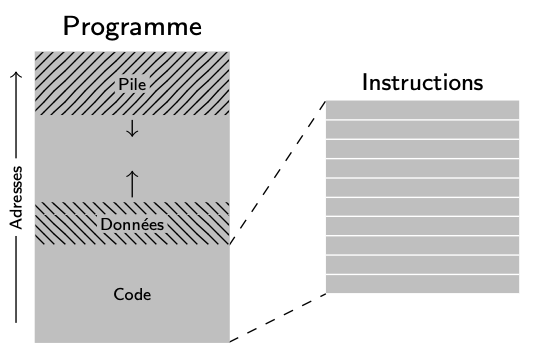
\includegraphics[width=0.4\textwidth]{Images/View/program-view.png}
    \caption{Program view}
\end{figure}

\subsection{Concept de base – évènement}

Lorsqu’un programme est exécuté par le processeur, deux questions se posent :
\begin{itemize}
    \item \textbf{Erreur d'instruction} : Doit-on redémarrer la machine ou gérer l’anomalie pour limiter les dégâts ?
    \item \textbf{Activité de périphérique externe} (e.g. frappe au clavier) : Peut-on suspendre temporairement le programme en cours pour traiter l’activité ?
\end{itemize}

Ces situations sont résolues par la gestion des \textbf{évènements}, mécanismes permettant au processeur de brancher vers du code spécifique en réponse à un évènement.

\subsection{Exceptions (évènements synchrones)}
Origine interne, résultant de l’exécution de l’instruction courante :
\begin{itemize}
    \item \textbf{Code opératoire invalide} : Opcode non reconnu par le processeur.
    \item \textbf{Division par zéro} : Nécessité d’un dénominateur non-nul.
    \item \textbf{Instruction privilégiée} : Niveau de privilège insuffisant pour exécuter l’instruction.
    \item \textbf{Instruction non-chargée en mémoire} : Le système d’exploitation charge la partie manquante en mémoire.
\end{itemize}

\subsection{Interruptions (évènements asynchrones)}
Origine externe, provoquées par un signal de périphérique :
\begin{itemize}
    \item \textbf{Frappe de clavier} : Fermeture d’un circuit électronique, générant une interruption.
    \item \textbf{Fichier prêt pour lecture} : Le contrôleur de disque génère une interruption après lecture des données.
    \item \textbf{Réception d’un paquet réseau} : La carte réseau génère une interruption après réception complète d’un paquet.
    \item \textbf{Erreur du matériel} : Anomalies détectées (e.g. température excessive).
    \item \textbf{Signal d’horloge} : Interruption générée 32.768 fois par seconde pour suivre le temps.
\end{itemize}


\subsection{Conséquences possibles pour le programme}

Le système d'exploitation doit gérer les évènements survenus pendant l'exécution d'un programme. Selon la nature de l'évènement, deux décisions peuvent être prises :

\begin{itemize}
    \item \textbf{Évènement récupérable} : Après traitement, il est possible de continuer l'exécution du programme.
    \item \textbf{Évènement irrécupérable} : La faute ne peut être corrigée, et il est nécessaire de terminer le programme.
\end{itemize}

\subsubsection{Evènement récupérable}

Lorsqu'un évènement récupérable survient, il est crucial de préserver l'état du processeur. Le gestionnaire d'évènements doit sauvegarder le contexte du programme suspendu (registres et stack) avant de traiter l'évènement. Cette sauvegarde est similaire à celle d'un appel de fonction.

% Le gestionnaire d'évènements sauvegarde uniquement les registres pertinents (e.g. $r_, $s_, $t_). Certaines architectures de processeur utilisent un mécanisme de basculement de stack pour éviter les interférences.

La continuation peut être :
\begin{itemize}
    \item \textbf{Reprise} : Retenter l'exécution de l'instruction qui a causé l'évènement.
    \item \textbf{Poursuite} : Passer à l'instruction suivante.
\end{itemize}

Les interruptions sont généralement des évènements récupérables avec poursuite, car elles n'affectent pas l'instruction en cours. Les exceptions comme les appels systèmes (e.g. \texttt{syscall}, \texttt{int}) sont également des évènements récupérables avec poursuite.

Par exemple, une interruption causée par une frappe au clavier est traitée en lisant le code de la touche depuis un port d'entrée/sortie, le traduisant en caractère, puis le transférant au programme destinataire, souvent la fenêtre active dans une interface graphique.

\subsubsection{Evènement irrécupérable}

Lorsqu'un évènement irrécupérable survient, le programme ne peut plus continuer. Une sauvegarde complète du contexte d'exécution est effectuée pour le débogage.

Le programme acquiert diverses ressources (mémoire, descripteurs de fichiers, sockets) au cours de son exécution. Ces ressources doivent être libérées lorsque le programme est terminé.

Les étapes de gestion d'un évènement irrécupérable incluent :
\begin{itemize}
    \item Affichage d'une notification à l'utilisateur décrivant le problème rencontré.
    \item Sauvegarde du contexte dans un fichier (e.g. \texttt{coredump}) ou envoi par mail à un serveur de rapports de crash.
    \item Libération du processeur, permettant la continuation d'un autre programme via un \textit{context switch}.
\end{itemize}


\subsection{Mécanismes de déroutement}

Chaque architecture de processeur spécifie et implémente son mécanisme de déroutement pour la gestion des évènements. Deux techniques principales sont utilisées :

\begin{itemize}
    \item \textbf{Déroutement avec registre de cause} : Un registre indique la cause de l'évènement, permettant au gestionnaire d'évènements de déterminer l'action appropriée.
    \item \textbf{Vectorisation} : Différents types d'évènements sont associés à des adresses spécifiques dans une table de vecteurs, chaque adresse pointant vers le code de gestion correspondant.
\end{itemize}

La technique utilisée influence l'organisation et les responsabilités du code du gestionnaire d'évènements.


\subsubsection{Registre de cause}

Le registre de cause encode les évènements survenus lors du cycle d’exécution courant, mettant à jour les bits pour les exceptions et interruptions. Si au moins un bit est positionné, le processeur réalise un déroutement vers une adresse précise.

Le gestionnaire d’évènements doit :
\begin{itemize}
    \item Lire le contenu du registre de cause.
    \item Tester et traiter les bits des interruptions en attente (bits à 1).
    \item Traiter les exceptions stipulées par le code d’exception.
\end{itemize}

Cette technique permet au système d’exploitation de déterminer l’ordre de priorité des traitements des différents évènements. La fonction principale du gestionnaire d’évènements doit être placée à l’adresse de déroutement définie par le processeur au démarrage du système.

Pour permettre la continuation du programme, l’adresse de l’indicateur d’instruction courante est sauvegardée dans un registre dédié (e.g. Exception Program Counter en MIPS32).


\subsubsection{Vectorisation}

Dans la vectorisation, chaque type d'évènement est associé à un numéro unique (e.g. interrupt vector). Ce numéro identifie une entrée dans une table de descripteurs (e.g. interrupt descriptor table, IDT) qui référence la fonction de traitement spécifique à invoquer (interrupt service routine, ISR). 

À la fin d’un cycle d’exécution, le processeur :
\begin{itemize}
    \item Consulte les numéros d’évènements survenus.
    \item Invoque les fonctions de gestion des évènements correspondantes dans un ordre déterminé.
\end{itemize}

Le code du gestionnaire d’évènements se concentre uniquement sur l’évènement correspondant. Au démarrage du système, l’OS initialise le contenu de la table des descripteurs et la référence au processeur via une instruction privilégiée (e.g. \texttt{lidt} en x86).

Lorsqu’un évènement survient :
\begin{itemize}
    \item Le numéro d’évènement sert d’indice dans l’IDT.
    \item Le descripteur correspondant (interrupt gate) contient l’adresse de la fonction de gestion vers laquelle brancher (offset).
\end{itemize}


\subsubsection{Niveaux de privilège}

Le jeu d'instructions d'un processeur inclut toutes les instructions reconnaissables par son architecture, comprenant les instructions arithmétiques, logiques et systèmes. 
Les instructions systèmes modifient la configuration du processeur et doivent être exécutées uniquement par le système d'exploitation.

Un niveau de privilège contrôle quelles instructions peuvent être exécutées et quand. 
La spécification du processeur décrit la dynamique de changement de ce niveau de privilège et son utilisation pour les vérifications. 

\subsubsection{Basculement de stack}

Lorsqu’un évènement survient, le processeur déroute vers une fonction du système d’exploitation, modifiant le contenu des registres et utilisant une stack pour stocker les valeurs temporaires. Il est crucial de décider si cette stack sera celle du programme suspendu ou une stack dédiée du système d’exploitation.

Le processeur peut basculer vers une stack du système d’exploitation, en sauvegardant les informations nécessaires pour explorer la stack du programme suspendu (e.g. stack pointer). Par exemple, lors d'un appel système, les arguments peuvent être passés via la stack, et le système d’exploitation doit pouvoir les localiser.

Après le traitement de l’évènement, la stack courante redevient celle du programme. La figure 1.11 illustre ce processus :
\begin{itemize}
    \item Avant le déroutement : \texttt{sp(pgm)}
    \item Après le déroutement : \texttt{sp(os)}, contenant :
    \begin{itemize}
        \item Sauvegarde du pointeur de stack précédent \texttt{sp(pgm)}
        \item Indicateur d’instruction courante \texttt{ip(pgm)}
        \item Éventuel code d’erreur décrivant l’évènement
    \end{itemize}
\end{itemize}

Ces informations permettent de revenir au programme pour une éventuelle continuation.



\subsection{Multiplicité des occurences}

Il est possible que plusieurs évènements se produisent pendant un même cycle d’exécution du processeur. 
Les règles d'agrégatioons entre événements sont les suivantes :

\begin{itemize}
    \item \textbf{Reprise} l’emporte sur une \textbf{poursuite}.
    \item \textbf{Abandon} l’emporte sur une \textbf{reprise}.
\end{itemize}

Lors de deux évènements similaires (deux poursuites, deux reprises, ou deux abandons), la conséquence est respectivement une poursuite, une reprise, ou un abandon.

Pour des évènements de types différents :
\begin{itemize}
    \item \textbf{Reprise et poursuite} : La reprise l’emporte, les deux traitements doivent être réalisés. Si l'évènement avec poursuite est une interruption, il peut être traité en priorité.
    \item \textbf{Poursuite et abandon} : L’abandon l’emporte. Si l'évènement avec poursuite est une exception, son traitement n'est pas nécessaire. Si c'est une interruption, il doit être traité.
    \item \textbf{Reprise et abandon} : L’abandon l’emporte. Le traitement de l'évènement avec reprise n'est pas nécessaire car le programme ne continuera plus.
\end{itemize}



\subsection{Gestion ré-entrante des évènements}

Un évènement peut survenir pendant n'importe quel cycle d'exécution, y compris pendant la gestion d'un autre évènement (exception ou interruption). Le gestionnaire d'évènements doit être adapté pour gérer cette imbrication correctement.

Un gestionnaire ré-entrant permet de gérer de nouveaux évènements survenant pendant l'exécution du gestionnaire actuel. Les considérations sont similaires à la gestion des appels de fonctions récursives. 

Pour garantir une sauvegarde cohérente des contextes imbriqués :
\begin{itemize}
    \item Utiliser la stack pour sauvegarder le contexte du gestionnaire d'évènements suspendu.
    \item Désactiver les interruptions pendant les phases critiques (sauvegarde du contexte, restauration du contexte, continuation), mettant ainsi en attente les interruptions.
    \item Préserver l'adresse de l'instruction corrélée à chaque niveau d'imbrication.
\end{itemize}

\subsection{Priorités et masques d'interruptions}

Dans un système typique, il est crucial de respecter l'ordre de priorité des interruptions. Un gestionnaire ré-entrant seul ne suffit pas pour éviter l'inversion de priorité, où une interruption de basse priorité pourrait interrompre le traitement d'une interruption de haute priorité.

La solution consiste à utiliser un masque d'interruptions, permettant une granularité dans l'activation et la désactivation des interruptions. Ce masque contrôle quelles interruptions sont actives (ou inactives) en utilisant un bit par type d'interruption. Le masque est combiné avec les bits des interruptions en attente à la fin de chaque cycle d'exécution.

Lors du traitement d'une interruption, le gestionnaire :
\begin{itemize}
    \item Positionne les bits du masque pour autoriser uniquement les interruptions plus prioritaires.
    \item Après traitement, restaure l'état du masque à son état précédent.
\end{itemize}



\newpage
\section{Mémoire}\label{sec:memoire}


\newpage
\section{Processus}\label{sec:processus}

\subsection{Problématique}
Un processus est une instance d'un programme en cours d'exécution, comprenant son code, ses données et ses ressources système allouées. 
La gestion des processus est essentielle pour assurer l'exécution efficace et sécurisée des programmes sur un système informatique.

\subsection{Constitution d'un processus}
Un processus se compose de plusieurs éléments :
\begin{itemize}
    \item \textbf{Espace d'adressage} : Comprend le code du programme, les données statiques, la pile et le tas.
    \item \textbf{Descripteur de processus} : Contient l'identifiant unique (PID), l'état, les registres, le pointeur de pile, et les descripteurs de fichiers ouverts.
\end{itemize}

\subsection{Cycle de vie d'un processus}
Le cycle de vie d'un processus inclut plusieurs états :
\begin{itemize}
    \item \textbf{Création} : Un processus parent crée un processus enfant via un appel système tel que fork().
    \item \textbf{Exécution} : Le processus utilise le processeur pour exécuter les instructions.
    \item \textbf{Prêt} : Le processus est en attente de l'allocation du processeur.
    \item \textbf{Bloqué} : Le processus attend qu'une condition soit remplie (e.g., fin d'I/O).
    \item \textbf{Terminaison} : Le processus libère ses ressources et passe à l'état zombi jusqu'à ce que son descripteur soit nettoyé par le processus parent.
\end{itemize}

\subsection{Ordonnancement des processus}
L'ordonnancement est la méthode utilisée par le système d'exploitation pour attribuer du temps processeur aux processus prêts à s'exécuter. 
Les principales politiques d'ordonnancement incluent :
\begin{itemize}
    \item \textbf{First-Come, First-Served (FCFS)} : Les processus sont exécutés dans l'ordre de leur arrivée.
    \item \textbf{Round-Robin} : Chaque processus reçoit un quantum de temps fixe pour s'exécuter tour à tour.
    \item \textbf{Shortest Job Next (SJN)} : Le processus avec le temps d'exécution le plus court est exécuté en premier.
\end{itemize}

\subsubsection{Systèmes batch}

Les systèmes batch exécutent des lots de travaux sans interaction avec avec l'utilisateur pendant l'exécution.

Algorithmes
\begin{itemize}
    \item First-Come, First-Served (FCFS): Les processus sont exécutés dans l'ordre de leur arrivée.
    \item Shortest Job Next (SJN): Les processus avec le plus court temps d'exécution sont prioritaires
\end{itemize}
\subsubsection{Systèmes interactifs}

Les systèmes interactifs permettent une interaction continue avec l'utilisateur, nécessitant des temps de réponse courts.

Algorithmes:
\begin{itemize}
    \item Round Robin: chaque processus reçoit un temps de CPU fixe, appelé quantum, et est ensuite placé à la fin de la file d'attente.
    \item Priority scheduling: les processus sont exécutés en fonction de leur priorité.
\end{itemize}
\subsubsection{Systèmes en temps réel}

Les systèmes en temps réels doivent répondre à des contraintes temporelles strictes, souvent utilisés dans des applications critiques.

Algorithmes:
\begin{itemize}
    \item Rate Monotonic Scheduling (RMS): les processus avec les périodes les plus courtes ont la plus haute priorité
    \item Earliest Deadline First (EDF) : Les processus sont exécutés en fonction de leur échéance la plus proche
\end{itemize}

\subsection{Multi-threading}
Le multi-threading permet à un processus de contenir plusieurs threads d'exécution, ce qui améliore l'efficacité et la réactivité. Les threads partagent l'espace d'adressage du processus mais possèdent des contextes d'exécution indépendants.

\subsection{Gestion des événements et des interruptions}
Les interruptions permettent de gérer des événements asynchrones (e.g., I/O). 
Lorsqu'une interruption se produit, le système d'exploitation sauvegarde le contexte du processus courant et exécute le gestionnaire d'interruption approprié.

\subsection{Conclusion}
La gestion des processus est fondamentale pour le fonctionnement d'un système d'exploitation, impactant directement l'efficacité et la stabilité des systèmes informatiques. 
Une bonne compréhension de la constitution des processus, de leur cycle de vie, des stratégies d'ordonnancement et du multi-threading est essentielle pour développer des applications performantes et robustes.


\newpage
\section{Concurrence}\label{sec:concurrence}

\subsection{Problématique}
La concurrence en informatique permet d'exécuter plusieurs processus ou threads simultanément, augmentant ainsi la réactivité et l'efficacité des systèmes. 
Toutefois, cette parallélisation introduit de nouveaux défis, notamment les conditions de course, l'exclusion mutuelle et les deadlocks.

\subsection{Mécanismes de communication}
Les processus et threads peuvent communiquer via plusieurs mécanismes :
\begin{itemize}
    \item \textbf{Mémoire partagée} : Utilisation d'une mémoire commune pour échanger des données.
    \item \textbf{Passage de messages} : Envoi de messages explicites entre processus ou threads.
    \item \textbf{Fichiers} : Utilisation de fichiers communs pour la lecture et l'écriture de données.
\end{itemize}

\subsection{Conditions de course}
Les conditions de course surviennent lorsque plusieurs threads accèdent simultanément à des données partagées sans synchronisation adéquate, entraînant des résultats imprévisibles. 
Pour les éviter, des mécanismes de synchronisation tels que les verrous (mutex) et les sémaphores sont utilisés.

\subsection{Sections critiques}
Une section critique est une portion de code qui doit être exécutée par un seul thread à la fois pour éviter les conditions de course. Les solutions incluent :
\begin{itemize}
    \item \textbf{Attente active} : Les threads vérifient continuellement une condition jusqu'à ce qu'elle soit vraie, ce qui peut être inefficace.
    \item \textbf{Blocage} : Les threads se mettent en attente jusqu'à ce qu'ils puissent entrer dans la section critique, ce qui est plus efficace que l'attente active.
\end{itemize}

\subsection{Problèmes classiques}
Les problèmes classiques de la concurrence comprennent :
\begin{itemize}
    \item \textbf{Producteur-consommateur} : Synchronisation entre un producteur qui crée des données et un consommateur qui les utilise.
    \item \textbf{Dîner des philosophes} : Un problème de synchronisation qui illustre les deadlocks et les solutions potentielles, comme l'utilisation de mutex.
\end{itemize}

\subsection{Deadlocks}
Un deadlock survient lorsque plusieurs threads se bloquent mutuellement en attente de ressources. 
Les conditions nécessaires pour un deadlock sont l'exclusion mutuelle, la possession et l'attente, l'absence de préemption, et la formation d'un cycle d'attente.

\subsection{Stratégies pour éviter les deadlocks}
Pour éviter les deadlocks, plusieurs stratégies peuvent être utilisées :
\begin{itemize}
    \item \textbf{Prévention} : Empêcher les conditions nécessaires au deadlock.
    \item \textbf{Évitement} : Utiliser des algorithmes pour éviter d'entrer dans des états de deadlock, comme l'algorithme du banquier.
    \item \textbf{Détection et récupération} : Détecter les deadlocks et prendre des mesures pour les résoudre.
\end{itemize}

\subsection{Conclusion}
La gestion de la concurrence est essentielle pour tirer parti du parallélisme et améliorer les performances des systèmes informatiques. 
Une compréhension approfondie des mécanismes de communication, des conditions de course, des sections critiques et des stratégies de prévention des deadlocks est cruciale pour développer des systèmes robustes


\newpage
\section{Systèmes de fichiers}\label{sec:systemesdefichiers}


\newpage
\section{Entrées et sorties}\label{sec:entreessorties}



\newpage
\appendix
% \section{Différence entre \acrshort{tls} et le chiffrement par clé}
% \begin{table}[htbp]
    \centering
    \begin{tabularx}{\textwidth}{
        >{\raggedright\arraybackslash}p{2cm} 
        >{\raggedright\arraybackslash}X 
        >{\raggedright\arraybackslash}X}
        \toprule
        \rowcolor[HTML]{EFEFEF}
        \textbf{}           & \textbf{TLS}                                                                      & \textbf{Chiffrement par clé} \\
        \midrule
        Nature              & Protocole de sécurité pour les communications réseau                              & Méthode pour chiffrer/déchiffrer des données \\
        \midrule
        Utilisation de clés & Utilise à la fois des clés symétriques et asymétriques                            & Peut utiliser des clés symétriques ou asymétriques \\
        \midrule
        Objectif principal  & Sécuriser des sessions ou connexions entières                                     & Sécuriser des données ou messages spécifiques \\
        \midrule
        Mise en œuvre       & Négocie les paramètres de chiffrement avant le transfert de données               & Appliqué aux données elles-mêmes, indépendamment du canal \\
        \midrule
        Applications        & Sécurisation du web (HTTPS), courrier électronique, messagerie instantanée, etc.  & Chiffrement de fichiers, communication sécurisée, authentification, signature numérique \\
        \bottomrule
    \end{tabularx}
    \caption{Comparaison entre \acrshort{tls} et le chiffrement par clé}
    \label{tab:TLSvsKeyEncryption}
\end{table}

% \section{Différents types d'attaques}
% \begin{longtable}{p{0.25\linewidth} p{0.7\linewidth}}
    \toprule
    \textbf{Attaque} & \textbf{Défense} \\
    \midrule
    Observation du trafic utilisateur & Le contenu à l'extrémité de l'utilisateur est crypté, bien que les connexions aux répondants puissent ne pas l'être. \\
    \addlinespace
    Corrélation de timing de bout en bout & \acrshort{tor} minimise mais ne cache pas complètement ces corrélations. \\
    \addlinespace
    Corrélation de la taille de bout en bout & La multiplexation des flux dans le même circuit limite cette corrélation à la granularité des cellules. \\
    \addlinespace
    Empreinte digitale de site web & Potentiellement effective contre Tor; des défenses supplémentaires pourraient inclure des stratégies de padding. \\
    \addlinespace
    Compromission de clés & La rotation périodique des clés limite la fenêtre d'opportunité pour ces attaques. \\
    \addlinespace
    Compromission d'un \acrshort{or} par itération & \acrshort{tor} protège contre ce scénario en éliminant rapidement les informations nécessaires pour compléter une telle attaque. \\
    \addlinespace
    Exécution d'un serveur de destination hostile & Les attaques de fin à fin deviennent plus faciles si l'adversaire peut induire les utilisateurs à se connecter à son serveur web. \\
    \addlinespace
    Exécution d'un \acrshort{or} hostile & Un \acrshort{or} isolé hostile peut créer des circuits à travers lui-même ou altérer des modèles de trafic. \\
    \addlinespace
    Introduire un timing dans les messages & \acrshort{tor} n'adresse pas directement ces attaques, mais elles ne sont qu'une version plus forte des attaques passives de timing. \\
    \addlinespace
    Attaques de tag & Les vérifications d'intégrité sur les cellules empêchent cette attaque. \\
    \addlinespace
    Remplacement de contenus de protocoles non authentifiés & Un nœud de sortie hostile peut usurper le serveur cible pour des protocoles non authentifiés. \\
    \addlinespace
    Attaques de replay & Non pertinentes pour Tor; la rediffusion d'un côté de la poignée de main entraîne une clé de session différente. \\
    \addlinespace
    Attaques contre les points de rendez-vous & Bob peut limiter la réception de requêtes via des tokens d'autorisation, et les points d'introduction peuvent être secrètement annoncés. \\
    \addlinespace
    Attaques contre les serveurs de répertoire & Si un serveur de répertoire est compromis, il peut partiellement influencer le répertoire final, mais une majorité est nécessaire pour inclure des \acrshort{or} compromis. \\
    \bottomrule
    \end{longtable}

\section{Latence et anonymat}
Dans les sytèmes de communication en réseau, le niveau d'anonymat est toujours corrélé avec le niveau de latence de ce système.

L'anonymat d'un client sur un réseau informatique lui confère l'intraçabilité de son activité en ligne.
Dans le cadre de \acrshort{tor}, cela est réalisé via le routage du trafic à travers plusieurs n\oe uds ou \acrfull{or}: chaque n\oe ud n'ayant connaissance que de son prédécesseur ainsi que de son successeur.

La latence - somme des délais - dans un réseau informatique désigne le temps écoulé entre l'envoi d'un paquet de données depuis une source et sa réception par la destination.
Dans le cadre de \acrshort{tor}, son accroissement s'explique d'une part par la répartition géographique globale des \acrshort{or} (\textit{cfr,} \acrfull{pd}) et d'autre part par les délais de chiffrement, déchiffrement qui surviennent à chaque \acrshort{or} (\textit{cfr,} \acrfull{td}).

Cette latence est donc un compromis nécessaire pour obtenir un niveau élevé d'anonymat et de sécurité, car elle rend plus difficile pour un observateur de corréler le trafic entrant et sortant.


\section{Menaces}\label{sec:ad}

Comme décrit tout au long de ce rapport, \acrshort{tor} assure l'anonymat de ses client, la non-vulnérabilité des données qu'ils transmettent ainsi que l'intraçabilité de leurs communications de bout en bout. 
La présente section s'attardera sur les différents types d'attaques recensées dans l'article ainsi que les axes de défenses mis en place dans \acrshort{tor}.
L'anonymat sera abordé au point \ref{subsubsec:passive} "\nameref{subsubsec:passive}", les aspects cryptographiques au point \ref{subsubsec:active} "\nameref{subsubsec:active}".
Les servrus de répertoires au point \ref{subsubsec:annuaire} "\nameref{subsubsec:annuaire}" et les point de rendez-vous au \ref{subsubsec:rdv} "\nameref{subsubsec:rdv}".

\subsection{Passive}\label{subsubsec:passive}

Les attaques passives concernent uniquement l'établissement de profils sur base d'analyses permettant ainsi de compromettre l'anonymat. 
Le tableau \ref{tab:ad-passive} "\nameref{tab:ad-passive}" ci-dessous présente les différents types d'attaques passives recensées dans l'article et y associe un axe de défense.
\begin{table}[htpb]
    \centering
    \begin{tabularx}{\textwidth}{
        >{\raggedright\arraybackslash}X
        % p{4.5cm}
        >{\raggedright\arraybackslash}X}
    \toprule
    \rowcolor[HTML]{EFEFEF}
    \textbf{Menace}                          & \textbf{Solution} \\ 
    \midrule
    Observation des profils de trafic         & Le multiplexage de traffics sur un même circuit empêche l'analyse précise de profils de trafics. \\
    \midrule
    Observation du contenu utilisateur       & Si la destination est un noeud hostile, l'usage de \gls{privoxy}\footnote{Un privoxy est un proxy logiciel conçu spécialement pour \acrshort{tor} qui nettoye les protocoles d'application.} permet de conserver l'anonymat du client. \\
    \midrule
    Distinguabilité des options               & En permettant aux utilisateurs de confugurer leurs profils, cela compromet leur anonymat. \\
    \midrule
    Corrélation temporelle de bout en bout   & Masquer la communication entre le \acrshort{op} et le premier \acrshort{or} via un \acrshort{op} sur le \acrshort{or}. Cela contraint à séparer le traffic en provenance du trafic traversant. \\
    \midrule
    Corrélation de taille de bout en bout    & Rembourage\footnote{nombre différent de paquets autorisés} ou topologie du tuyau fuyant\footnote{Le tuyau fuyant (leaky pipe) est une topologie de circuit utilisée dans le réseau Tor pour améliorer l'anonymat des utilisateurs. Dans cette configuration, le trafic peut être dirigé pour sortir du circuit à des nœuds intermédiaires plutôt qu'à la fin du circuit. }. \\
    \midrule
    Empreintes digitales de site Web         & Multiplexage des flux, modification de la taille des cellules et rembourages. \\
    \bottomrule
    \end{tabularx}
    \caption{Menaces et défenses dans \acrshort{tor} : attaques passives}
    \label{tab:ad-passive}
\end{table}

\newpage
\subsection{Active}\label{subsubsec:active}

Les attaqques actives concernent uniquement la compromission des techniques de chiffrement via divers procédés. 
Le tableau \ref{tab:ad-active} "\nameref{tab:ad-active}" ci-dessous présente les différents types d'attaques actives recencées dans l'article et y associe un axe de défense.
\begin{table}[htpb]
    \centering
    \begin{tabularx}{\textwidth}{
        >{\raggedright\arraybackslash}p{4.5cm}
        >{\raggedright\arraybackslash}X}
    \toprule
    \rowcolor[HTML]{EFEFEF}
    \textbf{Menace}                                         & \textbf{Solution} \\
    \midrule
    Compromission des clés                                  & La rotation periodique permet de contrer la compromission des clés de sessions \acrshort{tls} car même si l'attaquant peut observer les cellules relayées sur chacun des circuits de cette connexion, sans la clé oignon, il ne peut déchiffrer le contenu. \\ 
    \midrule
    Compromission itérative                                 & Le secret parfait vers l'avant (\textit{i.e.} Perfect Forward Secrecy) empêche de remonter un circuit même si un attaque a lieu d'un \acrshort{or} intermédiaire jusqu'au dernier. \\ 
    \midrule
    Exploitation d'un serveur web                           & \acrshort{tor} dépend de \gls{privoxy} pour empêcher un serveur web d'identifier des profils temporels des utilisateurs qui s'y connectent d'adapter ses réponses. \\
    \midrule
    Exploitation d'un proxy onion                           & À un client ne peut correspondre qu'un \acrshort{op} local. Cependant, compromettre un proxy onion compromet toutes ses connexions. \\ 
    \midrule
    Attaque DoS sur des nœuds non observables               & La mise en place de stratégies permettant au réseau de garder le contrôle sur les ressources matérielles utilisables permet de contrer les attaques de type Déni de service (\textit{i.e.} \acrfull{dos}). \\
    \midrule
    Exploitation d'un \acrshort{or} hostile                 & Un nœud hostile doit etre immediatement adjacent aux deux extremites pour compromettre l'anonymat d'un circuit. Si un adversaire contrôle plus d'un \acrshort{or}, il ne peut compromettre plus qu'une partie du trafic. \\ 
    \midrule
    Introduction de timing dans les messages                & Cela représente une version plus forte des attaques de timing passives déjà discutées. \\ 
    \midrule
    Attaques par marquage                                   & Les contrôles d'intégrité\footnote{Initialisation d'un digest SHA-1} sur les cellules empêchent un n\oe ud hostile de marquer une cellule en la modifiant. \\ 
    \midrule
    Remplacement de contenus de protocoles non authentifiés & La préférence des clients pour des protocoles authentifiés de bout en bout permet d'empêcher un nœud de sortie hostile de se faire passer pour le serveur cible. \\
    \midrule
    Attaques par rejeu                                      & Le protocole d'échnage de clés \acrshort{dh} permet de renégocier de nouvelles clés de session et ainsi contrer les attaques par replay. \\ 
    \midrule
    Attaques de diffamation                                 & Les politiques de sorties réduisent l'impact des attaques par diffamation. \\ 
    \midrule
    Distribution de code hostile                            & Des clés publiques de version officielles du code de \acrshort{tor} permettent de vérifier son authenticité avant de l'exécuter. \\ 
    \bottomrule
    \end{tabularx}
    \caption{Menaces et défenses dans \acrshort{tor} : attaques actives}
    \label{tab:ad-active}
\end{table}


\newpage
\subsection{Annuaire}\label{subsubsec:annuaire}
Les serveurs d'annuaires sont un coposante essentielle de tout réseau \acrshort{tor}.
% Le Tableau \ref{tab:structure-annuaire} "\nameref{tab:structure-annuaire}" ci-dessous reprend la structure ainsi que le contenu typique d'un annuaire.
% \begin{table}[htpb]
\centering
\begin{tabularx}{\textwidth}{
    >{\raggedright\arraybackslash}p{4cm}
    >{\raggedright\arraybackslash}p{3cm}
    >{\raggedright\arraybackslash}X}
\toprule
\textbf{Catégorie} & \textbf{Elément} & \textbf{Description} \\
\midrule
\textbf{Liste des Routeurs d'Oignons} & 
   \textbf{Identifiants} & Chaque routeur a une clé publique unique utilisée pour l'identifier. \\
   & \textbf{Adresses IP et Ports} & Les adresses réseau et les ports sur lesquels les routeurs écoutent. \\
   & \textbf{Politiques de Sortie} & Les types de trafic que les routeurs acceptent ou rejettent (par exemple, blocage de certains ports). \\
\midrule
\textbf{État des Routeurs} &
    \textbf{Disponibilité} & Indique si un routeur est actuellement en ligne et accessible. \\
    & \textbf{Capacités} & Bande passante disponible, latence, et autres métriques de performance.\\
    & \textbf{Charges de Travail} & Informations sur la charge actuelle et la capacité du routeur à gérer plus de trafic. \\
 & \\
\midrule
\textbf{Clés Cryptographiques} &
    \textbf{Clés d'Identité} & Clés publiques utilisées pour vérifier l'identité du routeur. \\
    & \textbf{Certificats} & Signatures numériques qui certifient l'authenticité des clés et des informations publiées. \\
 & \\
\midrule
\textbf{Descripteurs de Serveurs} &
    \textbf{Descriptions Signées} & Déclarations signées par les routeurs eux-mêmes, détaillant leur état et leurs capacités. \\
    & \textbf{Horodatages} & Indiquent le moment où les informations ont été mises à jour pour assurer leur fraîcheur. \\
 & \\
\midrule
\textbf{Informations de Réseau} &
    \textbf{Topologie} & Vue d'ensemble de la disposition et des connexions entre les routeurs dans le réseau. \\
    & \textbf{Consensus} & Ensemble de données consolidées approuvé par plusieurs serveurs d'annuaire pour garantir la cohérence et la fiabilité des informations. \\
 & \\
\bottomrule
\end{tabularx}
\caption{Structure et contenu d'un annuaire.}
\label{tab:structure-annuaire}
\end{table}

Les attaques contre les serveurs d'annuaires ciblent celles dont l'objectif est la compromission d'une partie des circuits créés.
Le tableau \ref{tab:ad-ds} "\nameref{tab:ad-rdvp}" ci-dessous présente les différents types d'attaques contre les serveurs d'annuaires et y associe un axe de défense.
\begin{table}[htpb]
    \centering
    \begin{tabularx}{\textwidth}{
        >{\raggedright\arraybackslash}p{4.5cm}
        >{\raggedright\arraybackslash}X}
    \toprule
    \rowcolor[HTML]{EFEFEF}
    \textbf{Menace}                                                         & \textbf{Solution} \\ 
    \midrule
    Destruction des serveurs d'annuaires                                    & Tant que la moitié des serveurs d'annuaires sont en activité, ils continuent de fournir un annuaire valide. \\
    \midrule
    Subversion d'un serveur d'annuaire                                      & N'a qu'une influence partielle et minime sur la composition de l'annuaire final. \\
    \midrule
    Subversion de la majorité des serveurs d'annuaire                       & Les opérateurs de serveurs d'annuaires doivent être indépendants et résistants. \\
    \midrule
    Encouragement à la dissension entre serveurs d'annuaire                 & Aucune solution n'est proposée pour empecher de diviser les opérateurs et ainsi leurs utilisateurs. \\
    \midrule
    Tromper les serveurs d'annuaire pour lister un \acrshort{or} hostile    & Les opérateurs de serveurs de annuaire sont capables de filtrer la plupart des \acrshort{or}s hostiles. \\
    \midrule
    Convaincre les annuaires qu'un \acrshort{or} défaillant fonctionne      & Les serveurs d'annuaires doivent impérativement tester les \acrshort{or} de manière appropriée pour empêcher qu'un \acrshort{or} ne puisse accepter une connexion \acrshort{tls} en ignorant les cellules et ainsi passer les barrières de sécurité de \acrshort{tor}. \\
    \bottomrule
    \end{tabularx}
    \caption{Menaces et défenses dans \acrshort{tor} : serveurs d'annuaires}
    \label{tab:ad-ds}
\end{table}


\subsection{Points de rendez-vous}\label{subsubsec:rdv}

Les attaques contre les points de rendez-vous.
Le tableau \ref{tab:ad-rdvp} "\nameref{tab:ad-rdvp}" ci-dessous recence les différent types d'attaques contre les points de rendez-vous et y associe un axe de défense.
\begin{table}[htpb]
    \centering
    \begin{tabularx}{\textwidth}{
        >{\raggedright\arraybackslash}p{4.5cm}
        >{\raggedright\arraybackslash}X}
            \toprule
            \rowcolor[HTML]{EFEFEF}
            \textbf{Menace}                         & \textbf{Solution} \\
            \midrule
            Multiples demandes d'introduction       & Les points de rendez-vous peuvent bloquer les requêtes qui ne contiennent pas de jetons d'autorisation, de restreindre le nombre de requêtes recevables ou d'exiger une certaine quantité de calcul pour chaque requête reçue. \\
            \midrule
            Attaquer un point d'introduction        & Désactiver les points de rendez-vous mais ils sont liés à des clés publiques.  \\
            \midrule
            Compromission d'un point d'introduction & Un point de rendez-vous compromis peut inonder le trafic ou empêcher de nouvelles demandes.  \\
            \midrule
            Compromission d'un point de rendez-vous & Trafic chiffré par une clé de session. \\
            \bottomrule
    \end{tabularx}
    \caption{Menaces et défenses dans \acrshort{tor} : points de rendez-vous}
    \label{tab:ad-rdvp}
\end{table}


\newpage
\renewcommand{\listfigurename}{Figures}
\listoffigures
\addcontentsline{toc}{section}{\listfigurename}

\newpage
\renewcommand{\listtablename}{Tableaux}
\listoftables
\addcontentsline{toc}{section}{\listtablename}

\newpage
\renewcommand{\listalgorithmname}{Algorithmes}
\listofalgorithms
\addcontentsline{toc}{section}{\listalgorithmname}

\newpage
\printglossary[title=Glossaire,toctitle=Glossaire]


\newpage
\printbibliography[title=Références]

\end{document}